\section{Data set}
\label{sec:data}

\begin{figure}[t]
	\centering
	\begin{subfigure}{.5\textwidth}
		\centering
		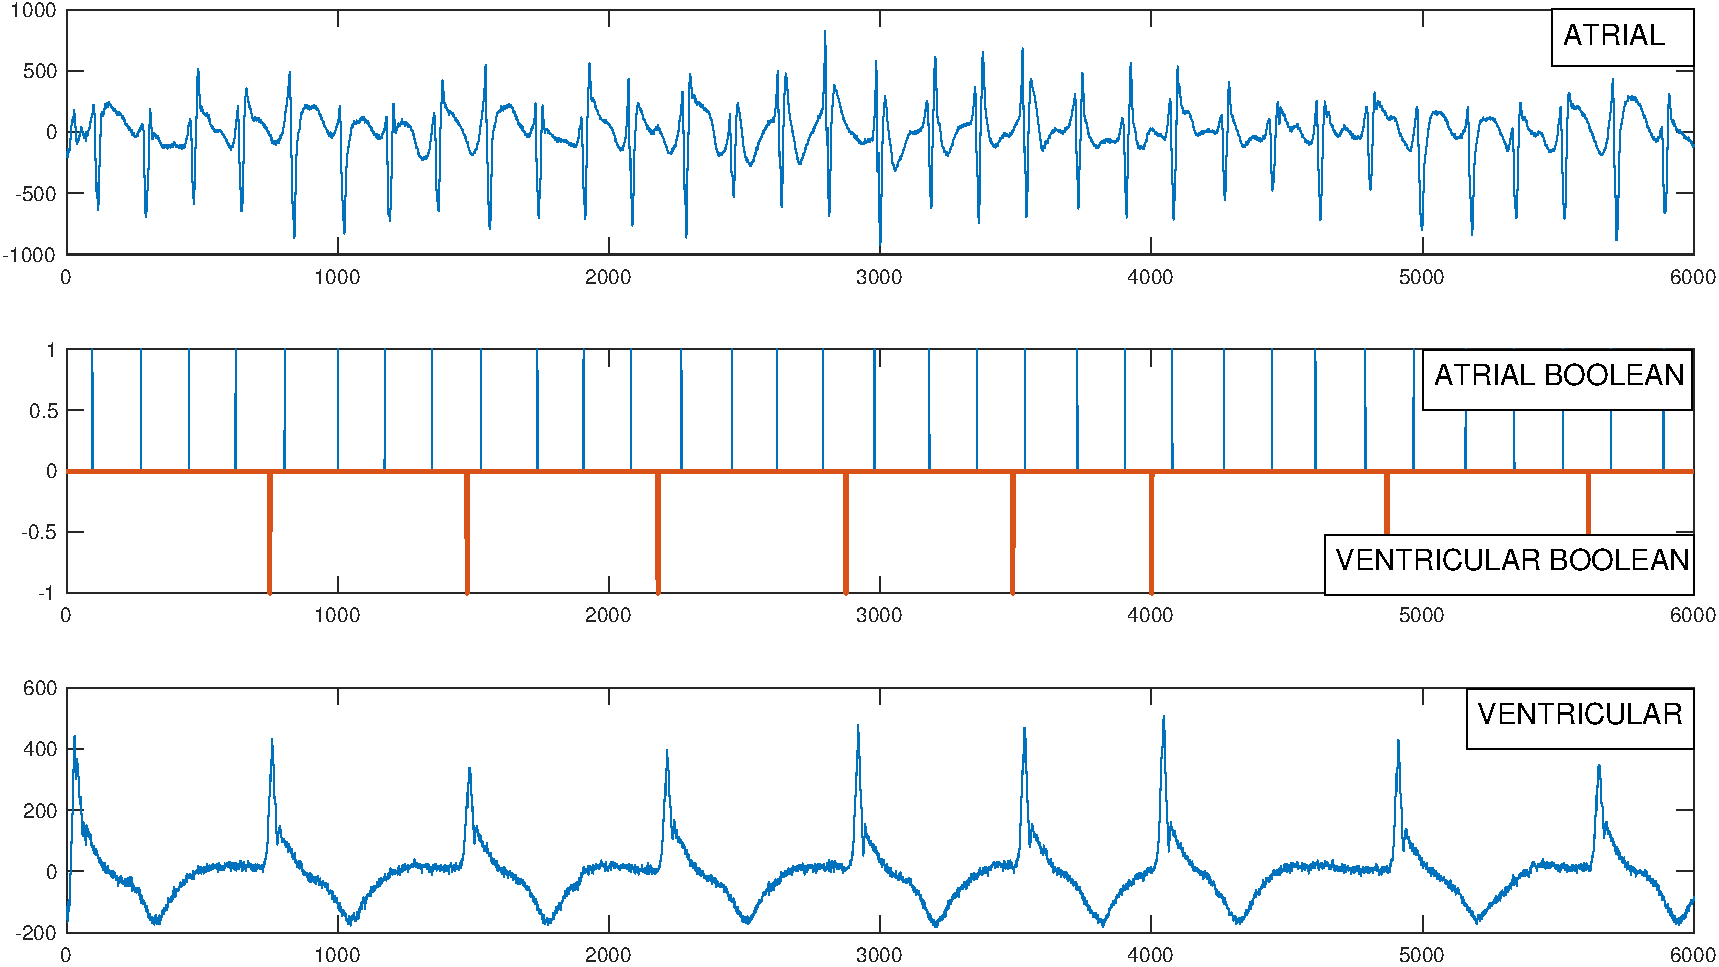
\includegraphics[scale=0.3]{figures/atachs.pdf}
		\caption{EGM recording during SVT. Bottom panel represents 
			V-signal, top 
			panel shows A-signal, middle panel presents corresponding 
			boolean beat channels.}
		\label{fig:egm}
	\end{subfigure}%
	\begin{subfigure}{.5\textwidth}
		\centering
		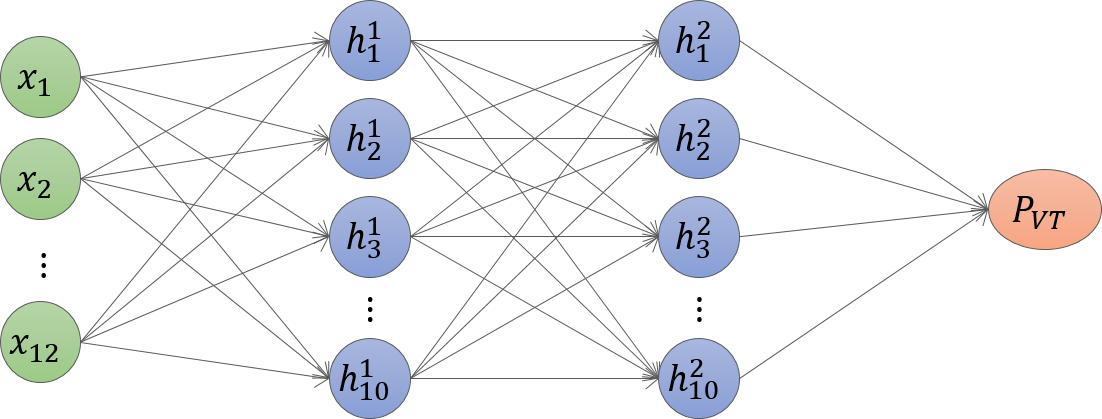
\includegraphics[width=0.95\textwidth]{figures/dnn_graph.png}
		\caption{DNN Model Architecture}
		\label{fig:dnn_graph}
	\end{subfigure}
	\caption{EGM signal example (left),	proposed DNN model (right).}
	\label{fig:yes}
\end{figure}





For our problem we used the  
%	\item \href{https://physionet.org/physiobank/database/mitdb/}{The 
%	MIT-BIH Arrhythmia Database}~\cite{moody2001impact}. 
%	It contains $48$ half-hour two-channel ECG recordings, obtained 
%	from $47$ subjects. The 
%	recordings are digitized at $360$ samples per second. 
%	There are approximately $110,000$ ECG
%	beats. 
%	in this database with $15$ different types of arrhythmia 
%including normal.
%	The subjects were 25 men aged 32 to 89 years, and 22 women aged 
%	23 to 89 years.
\textbf{Cardiac Model EGM Database}~\cite{jiang2016silico}. 
The EGM (electrogram) signals in the database were generated 
by the heart
model that has been validated for realism by 
cardiologists~\cite{jiang2016silico}.
	% EGM - cardiac device incoming cardiac voltage signal
	The database consists
	of $1920$ EGMs, equally split into $960$ VTs 
	and
	$960$ SVTs. Each recording has two real-valued channels, 
	depending on the 
	heart chamber where they were measured: Ventricular channel 
	(V-signal) and Atrial channel (A-signal). Each recording also has 
	two boolean channels, representing the detected heart beats in V- 
	and A-signals.
	
	An example SVT EGM recording is shown in a Figure~\ref{fig:egm}. 

%	\item Ann Arbor Electrogram Libraries~\cite{egm_data}. It 
%	consists of 89 EGM recordings: 62 VT signals and 27 SVT signals. 
%	Signals are of different length, varying from 10 seconds to 2 
%	minutes recordings. 
%\end{itemize}
\subsection{Data pre-processing and features extraction}
Following the methodology 
from~\cite{hajeb2018automated}, data pre-processing includes the 
following steps:
\begin{enumerate}
	\item Resample each signal with a sampling frequency of $300$Hz.
	\item Filter the signal with a fourth-order bandpass Butterworth 
	filter with low cut-off frequency of $0.4$Hz and high cut-off 
	frequency of $40$Hz to avoid baseline drift and reduce 
	high-frequency noise. 
	\item Segment the signal into $10$s data lengths.
	\item Extract 6 features from each signal (6 for each V-signal 
	and 6 for each A-signal: 12 in total): 
%	\begin{itemize}
%		\item Four features are derived 
%		from image-based phase plot analysis. These features 
%		represent nonlinear and non-stationary dynamics
%		of the signal, see~\cite{hajeb2018automated}.
%		\item One derived in the 
%		frequency domain, and is defined as a number of frequencies 
%		which have higher amplitude than the mean value.
%		\item One feature is Shannon 
%		Entropy~\cite{shannon1948mathematical} (The SE value is 
%		higher for VT than for SVT).
%	\end{itemize}
	four features are derived 
	from image-based phase plot analysis 
	(these features represent nonlinear and non-stationary dynamics
	of the signal, see~\cite{hajeb2018automated}), one derived in the 
	frequency domain (number of frequencies which have higher 
	amplitude than the mean value), and the last feature is Shannon 
	Entropy~\cite{shannon1948mathematical} (The SE value is higher 
	for VT than for SVT).
\end{enumerate}

%The feature extraction has transformed the complex ECG 
%signals into 12 features, which then leads to a success on forming 
%the classification problem. 
The final ML problem for our project is a 12-dimension-input binary 
classification problem.

%The first step of many algorithms that we will implement is feature 
%extraction. For ECG signals, those features can include, but not 
%limited to: signal amplitude, beat duration, signal segments and 
%waves durations, frequency domain features, short beats counter. 